\chapter{Xây dựng hệ thống }
% =======================
% PHẦN 1: SƠ ĐỒ KHỐI
% =======================
% =======================

\section{Sơ đồ khối hệ thống}

Hệ thống tổng quát chia ra hai thành phần chính: PC Side và PLC Side.  
Hai bên giao tiếp với nhau thông qua giao thức OPC UA.

\begin{figure}[h]
    \centering
    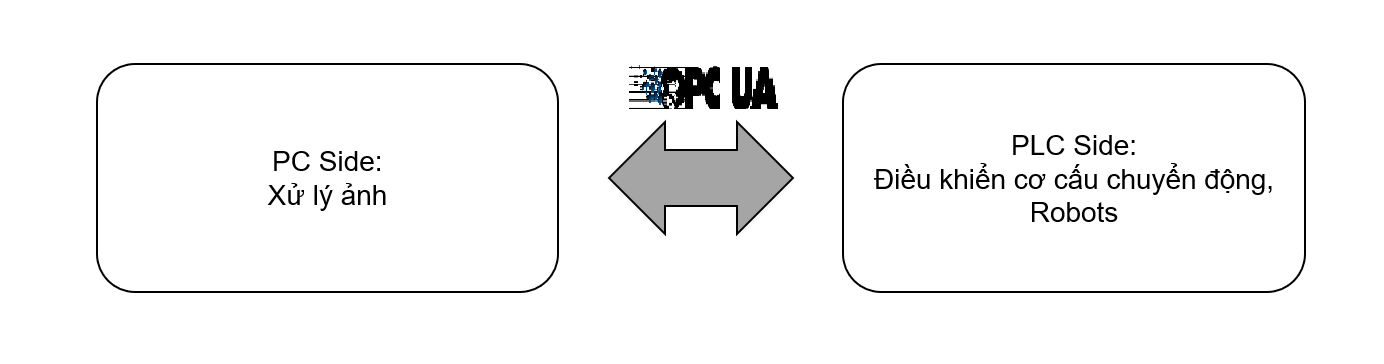
\includegraphics[width=1\textwidth]{figures/Chapter3/image1.png}
    \caption{Cấu trúc tổng quát hệ thống}
\end{figure}

\begin{enumerate}
    \item \textbf{PC Side:} 
    Máy tính đóng vai trò xử lý thị giác máy tính, chạy thuật toán phát hiện lỗi, phân loại NG/OK và trả kết quả về PLC thông qua OPC UA. Hệ thống bao gồm camera công nghiệp, phần mềm xử lý ảnh và module giao tiếp OPC UA Client. Cấu trúc hệ thống như Hình~\ref{c3:pcside}. 

    \begin{figure}[h]
        \centering
        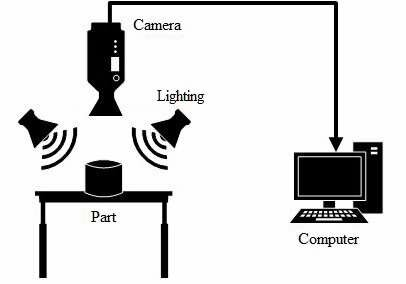
\includegraphics[width=0.5\textwidth]{figures/Chapter3/pcside.png}
        \caption{PC Side}
        \label{c3:pcside}
    \end{figure}

    \item \textbf{PLC Side:}  
    Hệ thống PLC bao gồm nguồn, CPU, module giao tiếp CC-Link (QJ61BT11N), module điều khiển chuyển động QD77MS16, màn hình HMI, các remote I/O, các trạm Robot, hệ thống servo và bộ khuếch đại.  
    Sơ đồ khối PLC Side được thể hiện trong Hình~\ref{c3:plcside}.

    \begin{figure}[h]
        \centering
        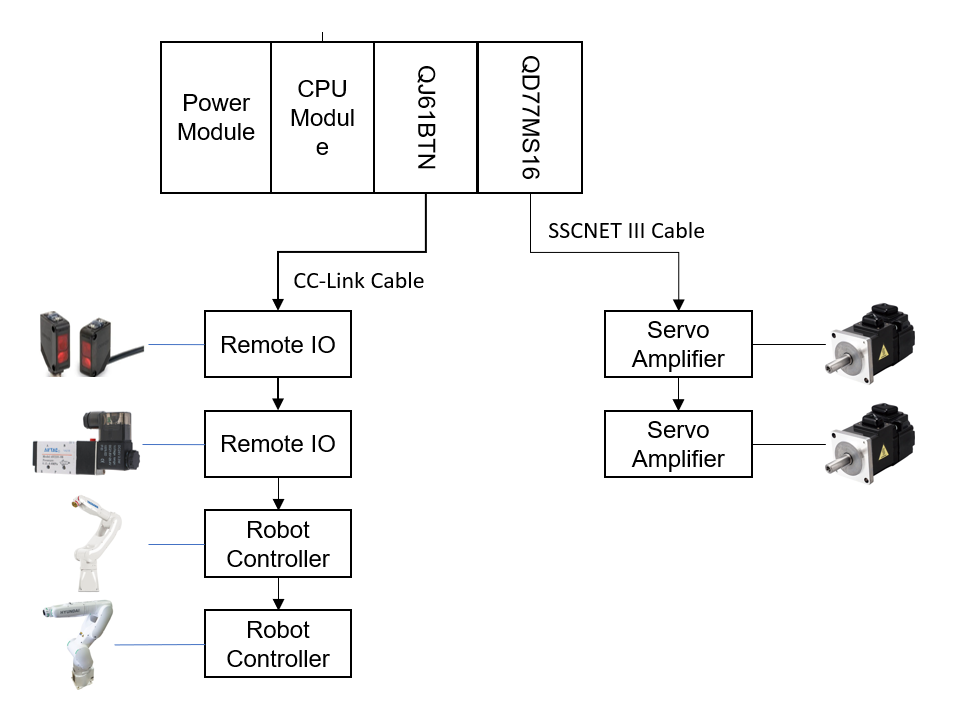
\includegraphics[width=1\textwidth]{figures/Chapter3/image2.png}
        \caption{PLC Side}
        \label{c3:plcside}
    \end{figure}

    \item \textbf{OPC UA:}  
    OPC UA (OPC Unified Architecture) được dùng để giao tiếp giữa PLC Side và PLC Side. 
\end{enumerate}


% =======================
% PHẦN 2: THUẬT TOÁN ĐIỀU KHIỂN
% =======================

